\documentclass[a4paper]{article}
\usepackage[utf8]{inputenc}
\usepackage[spanish, es-tabla, es-noshorthands]{babel}
\usepackage[table,xcdraw]{xcolor}
\usepackage[a4paper, footnotesep = 1cm, width=22cm, top=2.5cm, height=25cm, textwidth=20cm, textheight=25cm]{geometry}
%\geometry{showframe}

\usepackage{tikz}
\usepackage{amsmath}
\usepackage{amsfonts}
\usepackage{amssymb}
\usepackage{float}
\usepackage{graphicx}
\usepackage{caption}
\usepackage{subcaption}
\usepackage{multicol}
\usepackage{multirow}
\usepackage{wrapfig}
\setlength{\doublerulesep}{\arrayrulewidth}
\usepackage{booktabs}

\usepackage{hyperref}
\hypersetup{
    colorlinks=true,
    linkcolor=blue,
    filecolor=magenta,      
    urlcolor=blue,
    citecolor=blue,    
}

\newcommand{\note}[1]{
	\begin{center}
		\huge{ \textcolor{red}{#1} }
	\end{center}
}

\setcounter{topnumber}{2}
\setcounter{bottomnumber}{2}
\setcounter{totalnumber}{4}
\renewcommand{\topfraction}{0.85}
\renewcommand{\bottomfraction}{0.85}
\renewcommand{\textfraction}{0.15}
\renewcommand{\floatpagefraction}{0.8}
\renewcommand{\textfraction}{0.1}
\setlength{\floatsep}{5pt plus 2pt minus 2pt}
\setlength{\textfloatsep}{5pt plus 2pt minus 2pt}
\setlength{\intextsep}{5pt plus 2pt minus 2pt}

\newcommand{\quotes}[1]{``#1''}
\usepackage{array}
\newcolumntype{C}[1]{>{\centering\let\newline\\\arraybackslash\hspace{0pt}}m{#1}}
\usepackage[american]{circuitikz}
\usetikzlibrary{calc}
\usepackage{fancyhdr}
\usepackage{units} 

\graphicspath{{../Ejercicio-1/}{../Ejercicio-2/}{../Ejercicio-3/}{../Ejercicio-4/}{../ParteI/}{../ParteII/}{../ParteIII/}{../ParteIV/}}

\pagestyle{fancy}
\fancyhf{}
\lhead{22.14 - Electrónica IV}
\rhead{Mechoulam, Lambertucci, Londero}
\rfoot{Página \thepage}


\begin{document}

\subsection{Simulación de Curvas}

Para el estudio del modo discontinuo de la fuente estudiada anteriormente, se calculó la corriente media $I_{L_b} = I_{o_b}$ de boundary de la bobina, la cual es la misma que la corriente media de salida. El valor anterior de $\Delta I_L$ fue de $494.404mA$ por lo que la corriente media de boundary será

\begin{equation}
I_{L_b} = \frac{\Delta I_L}{2} = 247.202mA
\label{ej4:eq:il_boundary}
\end{equation}

Por esta razón, si la corriente de salida es menor que $I_{L_b}$, la fuente trabajará en modo discontinuo. Se seleccionó una resistencia de salida de $R_o = 500\Omega > R_{o_{min}} = \frac{V_o}{I_{L_b}} = 97.1\Omega$ para obtener resultados más significantes y se utilizó un duty cycle $D = 0.665$ para conservar los $24V$ de salida requeridos. A continuación se detallan las curvas simuladas.

\begin{figure}[H]
	\centering
	\begin{minipage}{0.495\textwidth}
		\centering
		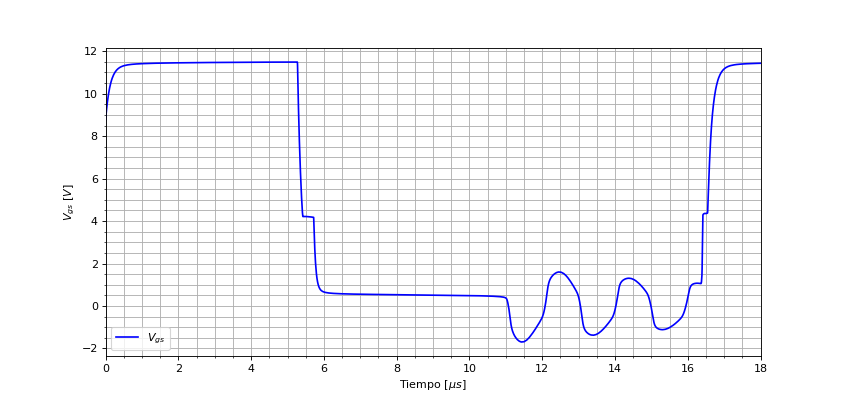
\includegraphics[width=\textwidth]{ImagenesEjercicio-4/vgs}% % first figure itself
		\caption{Tensión $V_{gs}$ en modo discontinuo.}
		\label{ej4:fig:vgs}
	\end{minipage}\hfill
	\begin{minipage}{0.495\textwidth}
		\centering
		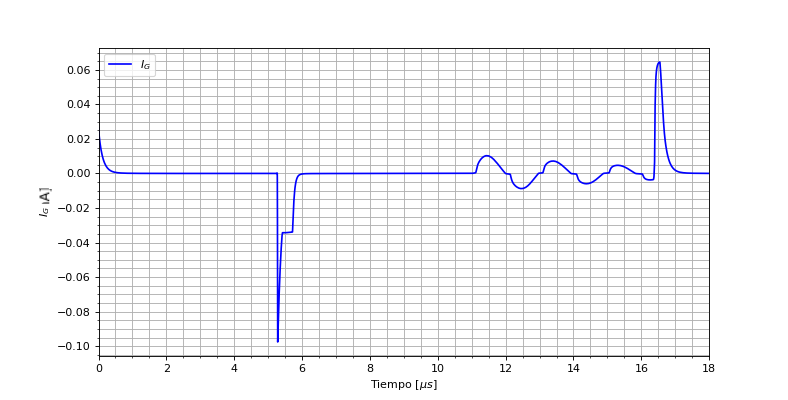
\includegraphics[width=\textwidth]{ImagenesEjercicio-4/ig} % second figure itself
		\caption{Corriente $I_{g}$ en modo discontinuo.}
		\label{ej4:fig:ig}
	\end{minipage}
\end{figure}

\begin{figure}[H]
	\centering
	\begin{minipage}{0.495\textwidth}
		\centering
		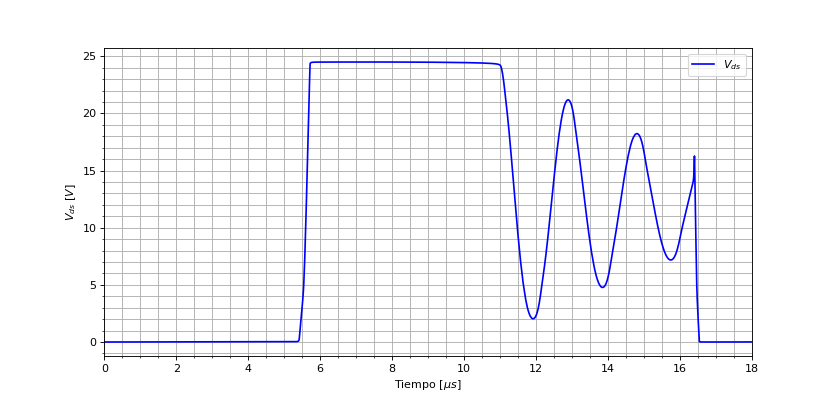
\includegraphics[width=\textwidth]{ImagenesEjercicio-4/vds} % first figure itself
		\caption{Tensión $V_{ds}$ en modo discontinuo.}
		\label{ej4:fig:vds}
	\end{minipage}\hfill
	\begin{minipage}{0.495\textwidth}
		\centering
		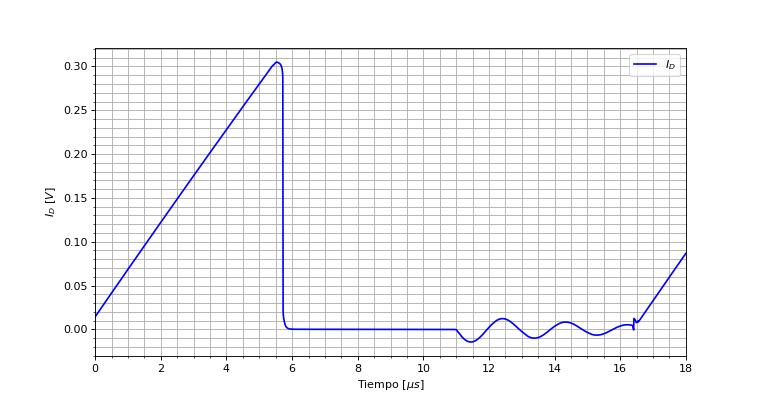
\includegraphics[width=\textwidth]{ImagenesEjercicio-4/id} % second figure itself
		\caption{Corriente $I_{D}$ en modo discontinuo.}
		\label{ej4:fig:id}
	\end{minipage}
\end{figure} 

\begin{figure}[H]
	\centering
	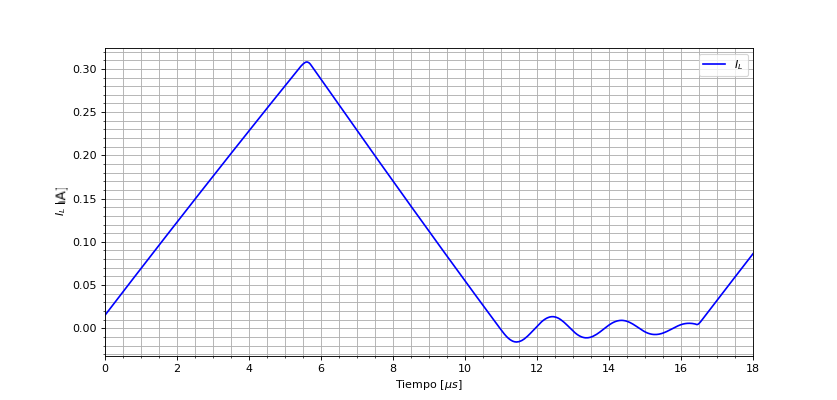
\includegraphics[width=0.7\linewidth, page=1]{ImagenesEjercicio-4/il}
	\caption{Corriente de la bobina en modo discontinuo.}
	\label{ej4:fig:il}
\end{figure}

A primera vista, lo que más llama la atención es la oscilación de $517KHz$ producida en el nodo compartido por la bobina, el switch y el diodo. Esto ocurre en el momento en el que se acaba la energía almacenada en el campo magnético. Este efecto de ringing es ocasionado debido a que, cuando la bobina queda sin energía y la corriente llega a cero, inductancias parásitas del circuito ocasionan que se genere una pequeña corriente $I_{rr}$ de inversa del diodo antes de que este se polarice en inversa, energizando a su vez un circuito RLC muy subamortiguado entre la bobina, el resistor de la bobina y los capacitores parasíticos del MOSFET. Este ringing producido por efectos parásitos puede resultar dañino para el transistor, si los picos de tensión sobrepasan la tensión máxima $V_{ds}$ de este. Además, estas oscilaciones pueden provocar emisiones electromagnéticas, reducir la eficiencia del convertidor a causa de disipación elevada de potencia, e incluso generar un ripple de tensión $\Delta V_o$ mayor a la salida, si se comienza un nuevo ciclo de carga de la bobina cuando la corriente de esta no cruza exactamente por el cero, como se observa en la Figura (\ref{ej4:fig:id}) [\href{https://www.researchgate.net/publication/317525001_Impact_of_inductor_current_ringing_in_DCM_on_output_voltage_of_DC-DC_buck_power_converters}{Impact of Inductor Current Ringing in DCM on Output Voltage of DC-DC Buck Power Converters}].

Una forma de reducir estas oscilaciones es implementando un circuito snubber [\href{https://www.ti.com/lit/an/slva255/slva255.pdf}{Minimizing Ringing at the Switch Node of a Boost Converter}] correctamente dimensionado a costo de aumentar la disipación de potencia y el tiempo de conmutación. Sabiendo que la pseudo-frecuencia de oscilación es de $f_{o} = 517KHz$ y aproximando la capacidad parásita $C_{par}$ que interactúa en el proceso como la capacidad parásita $C_{gd_1}$ se tiene que

\begin{equation}
	L_{par} = \frac{1}{C_{par}\left( 2\pi f_{o} \right)^2} = \frac{1}{750pf\left( 2\pi 517KHz \right)^2} = 126.3\mu H 
\end{equation}

Luego,

\begin{equation}
	C_{snub} = 3C_{par} = 2.225nF
\end{equation}

\begin{equation}
	R_{snub} = \sqrt{\frac{L_{par}}{C_{snub}}} = 355\Omega
\end{equation}

%Quedando el circuito como se observa en la Figura (). A continuación se detallan las curvas simuladas con el snubber en las Figuras (\ref{ej4:fig:vds_snub}) y (\ref{ej4:fig:il_snub}).
%
%\begin{figure}[H]
%	\centering
%	\begin{minipage}{0.495\textwidth}
%		\centering
%		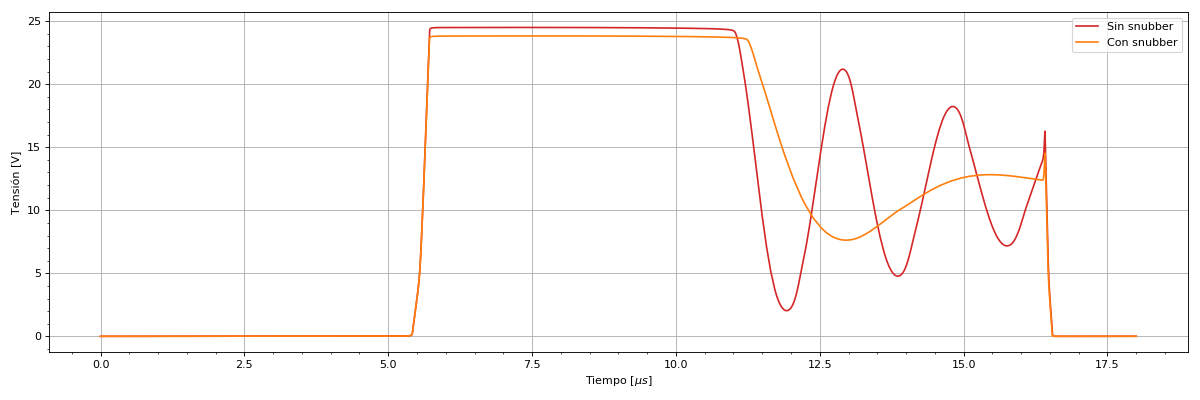
\includegraphics[width=\textwidth]{ImagenesEjercicio-4/comparacion-vds}	% first figure itself
%		\caption{Comparación entre $V_{ds}$ en modo discontinuo con y sin snubber.}
%		\label{ej4:fig:vds_snub}
%	\end{minipage}\hfill
%	\begin{minipage}{0.495\textwidth}
%		\centering
%		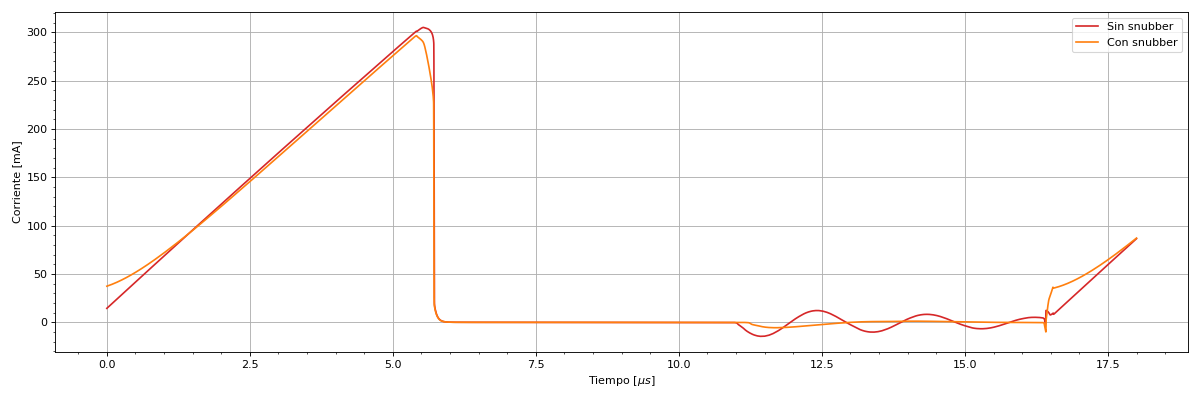
\includegraphics[width=\textwidth]{ImagenesEjercicio-4/comparacion-ids}	% second figure itself
%		\caption{Comparación entre $I_{ds}$ en modo discontinuo con y sin snubber.}
%		\label{ej4:fig:il_snub}
%	\end{minipage}
%\end{figure}

Quedando el circuito como se observa en la Figura (). A continuación se detallan las curvas simuladas con el snubber en la Figura (\ref{ej4:fig:vds_ids_snub}).

\begin{figure}[H]
	\centering
	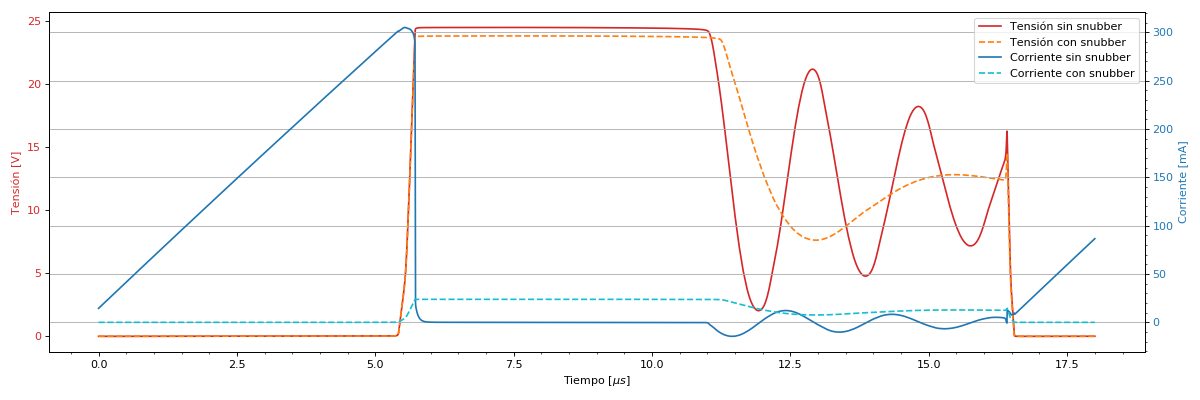
\includegraphics[width=0.9\linewidth]{ImagenesEjercicio-4/con-y-sin-snubber}
	\caption{Comparación de las curvas de $V_{ds}$ e $I_{ds}$ en modo discontinuo con y sin snubber.}
	\label{ej4:fig:vds_ids_snub}
\end{figure}

Si bien se puede observar una disminución en la amplitud y pseudo-frecuencia de oscilación, se puede sintonizar el circuito snubber más allá de los cálculos teóricos para lograr un mayor amortiguamiento. En la siguiente sección veremos como si bien este circuito logra disminuir el efecto de ringing, también aumenta la disipación de potencia.

\subsection{Potencia Disipada}

Se observa en la Figura () que para el encendido del MOSFET la potencia disipada fue disminuída considerablemente mientras que además ha disminuído la potencia en el apagado. 

\end{document}